%%
%% This is file `mcmthesis-demo.tex',
%% generated with the docstrip utility.
%%
%% The original source files were:
%%
%% mcmthesis.dtx  (with options: `demo')
%% 
%% -----------------------------------
%% 
%% This is a generated file.
%% 
%% Copyright (C)
%%     2010 -- 2015    by Zhaoli Wang
%%     2014 -- present by Liam Huang
%% 
%% This work may be distributed and/or modified under the
%% conditions of the LaTeX Project Public License, either version 1.3
%% of this license or (at your option) any later version.
%% The latest version of this license is in
%%   http://www.latex-project.org/lppl.txt
%% and version 1.3 or later is part of all distributions of LaTeX
%% version 2005/12/01 or later.
%% 
%% This work has the LPPL maintenance status `maintained'.
%% 
%% The Current Maintainer of this work is Liam Huang.
%% 
\documentclass{mcmthesis}
\mcmsetup{CTeX = false,   % 使用 CTeX 套装时,设置为 true
        tcn = 2001560, problem = C,
        sheet = true, titleinsheet = true, keywordsinsheet = false,
        titlepage = false, abstract = true}
\usepackage{palatino}
\usepackage{lipsum}

% \title{A Wealth of Data}
% \author{\small \href{http://www.latexstudio.net/}
%   {
\includegraphics[width=7cm]{mcmthesis-logo}}}
\date{\today}

\usepackage{geometry}
\geometry{left=1in,right=0.75in,top=1in,bottom=1in}
\usepackage{lastpage}

%%%%%%%%%%%%%%%%%%%%%%%%%%%%%%%%%%%%%%%%
\newcommand{\Problem}{C}    % 换成你的题号
\newcommand{\Team}{2001560} % 换成你的队号
%%%%%%%%%%%%%%%%%%%%%%%%%%%%%%%%%%%%%%%%

\begin{document}

\thispagestyle{empty}
\vspace*{-16ex}
\centerline{\begin{tabular}{*3{c}}
	\parbox[t]{0.3\linewidth}{\begin{center}\textbf{Problem Chosen}\\ \Large \textcolor{red}{\Problem}\end{center}}
	& \parbox[t]{0.3\linewidth}{\begin{center}\textbf{2020\\ MCM/ICM\\ Summary Sheet}\end{center}}
	& \parbox[t]{0.3\linewidth}{\begin{center}\textbf{Team Control Number}\\ \Large \textcolor{red}{\Team}\end{center}}	\\
	\hline
\end{tabular}}
%%%%%%%%%%% Begin Summary %%%%%%%%%%%

\vspace{2em}
\begin{center}
\Large\bf Title of you paper   % 论文标题
\end{center}

From here, begin your summary  % 摘要

%%%%%%%%%%% End Summary %%%%%%%%%%%

\clearpage
\pagestyle{fancy}
% Uncomment the next line to generate a Table of Contents
%\tableofcontents 
\newpage
\setcounter{page}{1}
\rhead{Page \thepage\ of \pageref{LastPage}}

\tableofcontents
\newpage

% \begin{abstract}
%   \lipsum[1]
% \end{abstract}
% \maketitle
%%
%% Generate the Memorandum, if it's needed.
\memoto{Marketing Director of Sunshine Company}
\memofrom{MCM Team \#2001560}
\memosubject{Data Analysis Results}
\memodate{\today}
% \logo{\LARGE I'm pretending to be a LOGO!}
\begin{memo}[Letter]
  \lipsum[1]
\end{memo}

\section{Introduction}
\subsection{Background}
In recent years, quantities of customers prefer to shopping online for its less spacetime limitation and the convenient home delivery service. However, compared to the traditional physical stores, customers can only evaluate products by the provided profile and pictures instead of seeing or testing the real ones. The information gap here is one of the leading causes of dissatisfied purchases. To help customers know the product better, many online marketplace platforms, such as Amazon, launch a "review system". Customers can express their level of satisfaction and further opinions or information about purchases through rating and reviewing. That additional information can help not only other customers make purchasing decisions, but companies improve the pros and cons of product design.\\

However, we found that not all reviews are equally relevant. Some reviews are too general; some people's ratings do not match their reviews; there are even deliberately misleading reviews, such as malicious defamation from competitors or the raise by the bribed reviewers. Therefore, when using data to assist business decisions, we need to analyze data carefully and comprehensively to obtain more accurate results. More factors should be considered, such as the ratings, review contents and review time, rather than straightly calculate the average rating level.

\subsection{Problem Restatement}
Analyze the three product data sets to describe quantitative and/or qualitative patterns, relationships that help evaluate a product's star ratings, reviews and helpfulness ratings. Use data to demonstrate that they are valuable.\\

Solve the following issues through modelling:
\begin{itemize}
  \item Determine the most informative metric based on ratings and reviews. This metric can track the product ratings of three products when they are on the market.
  
  \item Analyze the relationship between product ratings and time in three data sets.
  
  \item Look for critical factors that can affect the inflexion point of product ratings through time.
  
  \item Analyze whether there will be more a series of positive or negative reviews over a while and whether customer star ratings will be affected by recent reviews.
  
  \item Whether star rating and the keyword of review content match.
\end{itemize}

\subsection{Data}
\subsubsection{Data Source}
Our model is informed by the customer-supplied ratings and reviews for microwave ovens, baby pacifiers, and hair dryers sold in the Amazon marketplace over more than ten years.
\subsubsection{Data Pre-processing}
We did the following to sanitize the data set:
\begin{itemize}
  \item Remove factors that were not measured at all, such as marketplace and product category, for they can not present any information.
  
  \item Remove the redundant factors, such as review\_id and product\_id, for they can be completely replaced by customer\_id and product\_parent.
  
  \item Remove factors that could mislead the model, such as verify\_purchase ==N.
  
  \item Remove some garbled character.
\end{itemize}

\section{Assumptions}
\begin{itemize}
  \item Merchant's purpose: Guide users to buy products with quality reviews and recent reviews.
\end{itemize}
\begin{itemize}
  \item The content of the review and the star rating should be the same. People believe in reviews when review content is inconsistent with star ratings.

Reason: Based on popular psychology, real language is convincing 
\end{itemize}
\begin{itemize}
  \item Amazon Vine members' reviews are credible, excluding subjective factors that give high ratings for free products

Reason: Big data select Amazon Vine members. Their evaluations are more objective and practical.
\end{itemize}
\begin{itemize}
  \item Actual purchasers' reviews are credible.

Reason: People who have already experienced the product know more about the actual performance of the product.
\end{itemize}
\begin{itemize}
  \item Comments from actual non-purchasers are untrustworthy.

Reason: We listed the distribution of 1-5 stars between the non-purchasers and the purchasers. It shows that the non-purchasers give more 1 star than purchasers, which may mislead the reviews.

- fig1+2
\end{itemize}
\begin{itemize}
  \item The impact of the same purchaser on reviews is not taken into consideration; that is, each evaluation behaviour of the purchaser is independent and not related to the previous reviews.
\end{itemize}

\section{Nomenclature}
\begin{table}[h]
  \centering
  \begin{tabular}{ccc}
    \hline
    Symbol & Definition\\
    \hline
    star$_{i}$ & star rating of a review i\\
    
    ER$_{i}$ & emtional rating of a review i\\
      
    d$_{i}$ & the variance between star rating and emtional rating of a review i\\

    L$_{i}$ & length of a review i\\

    Vm$_{i}$ & whether a review i is from an Amazon vine member\\
      
    Vr$_{i}$ & votes rating of a review i\\
      
    M$_{i}$ & rating of a review i\\

    Q$_{i}$ & quality of a review i\\
          
    R$_{i}$ & synthesize evaluation of a review i\\
    
    R & average review synthesize evaluation\\
      
    t & time\\
    \hline
  \end{tabular}
  \caption{variables and functions}
\end{table}

\section{ Model Design }

\section{ Part \uppercase\expandafter{\romannumeral1}:  Rating Model based on star-ratings and reviews}

\section{ Part \uppercase\expandafter{\romannumeral2}:  Synthesize Evaluation Model}

\section{Sensitivity Analysis}

\section{Strengths and Weaknesses}
\subsection{Strengths}
\begin{itemize}
  \item \textbf{Applies widely}\\
        This  system can be used for many types of airplanes, and it also
        solves the interference during  the procedure of the boarding
        airplane,as described above we can get to the  optimization
        boarding time.We also know that all the service is automate.
  \item \textbf{Improve the quality of the airport service}\\
        Balancing the cost of the cost and the benefit, it will bring in
        more convenient  for airport and passengers.It also saves many
        human resources for the airline. \item \textbf{}
\end{itemize}
\subsection{Weaknesses and Improvement}
\begin{itemize}
  \item The small dataset causes deviation of the model which build by either word frequency analysis or LDA.
\end{itemize}
\begin{itemize}
  \item The LDA model has an excellent performance with document collection, while the majority of reviews are short in words. 
\end{itemize}
\begin{itemize}
  \item While major reviewers are not Amazon Vine Member, different people may have different criteria for evaluation, which may produce an objective assessment. We need to study every reviewers' rating habit to get a weight for every reviewer.
\end{itemize}
\begin{itemize}
  \item Removing the non-purchasers' reviews helps analysis the problem; however, these misleading reviews may hurt the customers' purchasing decisions and further ratings.
\end{itemize}

\section{Conclusions}

\begin{figure}[h]
  \small
  \centering
  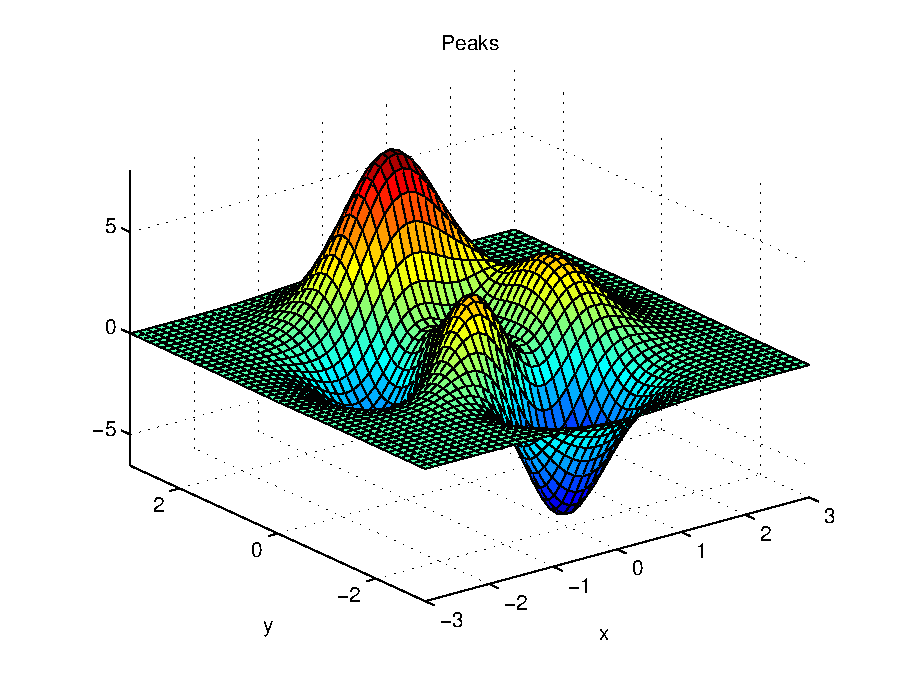
\includegraphics[width=12cm]{mcmthesis-aaa.eps}
  \caption{aa} \label{fig:aa}
\end{figure}

\lipsum[8] \eqref{aa}
\begin{equation}
  a^2 \label{aa}
\end{equation}


\[
  p_{j}=\begin{cases} 0,              & \text{if $j$ is odd}  \\
    r!\,(-1)^{j/2}, & \text{if $j$ is even}
  \end{cases}
\]

%% References
\begin{thebibliography}{99}
  \bibitem{1} D.~E. KNUTH   The \TeX{}book  the American
  Mathematical Society and Addison-Wesley
  Publishing Company , 1984-1986.
  \bibitem{2}Lamport, Leslie,  \LaTeX{}: `` A Document Preparation System '',
  Addison-Wesley Publishing Company, 1986.
  \bibitem{3}\url{http://www.latexstudio.net/}
  \bibitem{4}\url{http://www.chinatex.org/}
\end{thebibliography}

\begin{appendices}

  \section{First appendix}

  \lipsum[13]

  Here are simulation programmes we used in our model as follow.\\

  \textbf{\textcolor[rgb]{0.98,0.00,0.00}{Input matlab source:}}
  \lstinputlisting[language=Matlab]{./code/mcmthesis-matlab1.m}

  \section{Second appendix}

  some more text \textcolor[rgb]{0.98,0.00,0.00}{\textbf{Input C++ source:}}
  \lstinputlisting[language=C++]{./code/mcmthesis-sudoku.cpp}

\end{appendices}
\end{document}

%% 
%% This work consists of these files mcmthesis.dtx,
%%                                   figures/ and
%%                                   code/,
%% and the derived files             mcmthesis.cls,
%%                                   mcmthesis-demo.tex,
%%                                   README,
%%                                   LICENSE,
%%                                   mcmthesis.pdf and
%%                                   mcmthesis-demo.pdf.
%%
%% End of file `mcmthesis-demo.tex'.
